\chapter{ACID Test}
\label{sec:acid-test}

\newcommand{\bl}[1]{\textcolor{blue}{#1}}
\newcommand{\rd}[1]{\textcolor{red}{#1}}
\newcommand{\gn}[1]{\textcolor{green}{#1}}
\newcommand{\gy}[1]{\textcolor{grey}{\textit{#1}}}

\newcommand{\level}[1]{\textsf{#1}}
\newcommand{\anomaly}[1]{\rd{#1}}
\newcommand{\anolong}[1]{\emph{\rd{#1}}}
\newcommand{\tx}[1]{#1}

\newcommand{\cmark}{\ding{51}}
\newcommand{\xmark}{\ding{55}}


\begin{quote}
  \textit{This chapter is based on the chapter on "ACID tests" in the 
          \ldbcsnb(LDBC SNB specification).The main difference between
          this section and \ldbcsnb\xspace is the schema design. The
          framework and reference implementations of the ACID test suite
          are available at \url{https://github.com/ldbc/ldbc_finbench_acid}.
  }
\end{quote}

Verifying ACID compliance is an important step in the benchmarking process for 
enabling fair comparison between systems. The performance benefits of operating
with weaker safety guarantees are well established~\cite{DBLP:conf/ds/GrayLPT76}
but this can come at the cost of application correctness. To enable apples vs. 
apples performance comparisons between systems it is expected they uphold the 
ACID properties. Currently, LDBC provides no mechanism for validating ACID 
compliance within the FinBench Transaction workflow.

This chapter presents the design of an implementation-agnostic ACID-compliance
test suite for the Transaction workload\footnote{We acknowledge verifying 
ACID-compliance with a finite set of tests is not possible. However, the goal is
not an exhaustive quality assurance test of a system's safety properties but 
rather to demonstrate that ACID guarantees are supported.}. Our guiding design
principle was to be agnostic of system-level implementation details, relying 
solely on client observations to determine the occurrence of non-transactional 
behaviour. Thus all systems can be subjected to the same tests and fair 
comparisons between FinBench Transaction performance results can be drawn. Tests
are described in the context of a graph database employing the property graph data 
model~\cite{DBLP:journals/csur/AnglesABHRV17}. Reference implementations are 
given in Cypher~\cite{DBLP:conf/sigmod/FrancisGGLLMPRS18}, the \emph{de facto} 
standard graph query language.

Particular emphasis is given to testing isolation, covering 10~known anomalies.
A conscious decision was made to keep tests relatively lightweight, as to not 
add significant overhead to the benchmarking process.

\section{Background}

The tests presented in this chapter are defined on a small core of LDBC FinBench
schema given in \autoref{figure:core-schema}.

\begin{figure}[htbp]
    \centering
    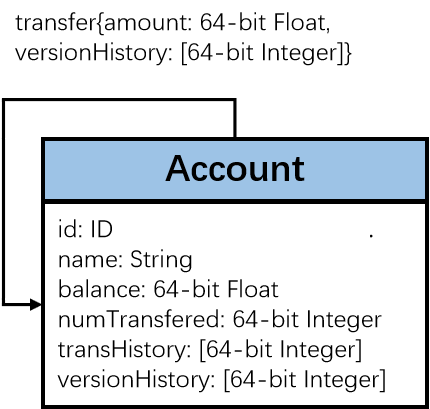
\includegraphics[scale=0.5]{figures/acid/acid-schema}
    \caption{Graph schema for the ACID test queries}
    \label{figure:core-schema}
\end{figure}

\begin{figure}[h]
  \centering
  \input{figures/acid/bailis}
\end{figure}

\section{Atomicity}

\emph{Atomicity} ensures that either all of a transaction's actions are 
performed, or none are. Two atomicity tests have been designed.

{\flushleft \textbf{Atomicity-C}} checks for every successful commit message a
client receives that any data items inserted or modified are subsequently visible.

{\flushleft \textbf{Atomicity-RB}} checks for every aborted transaction that all
its modifications are not visible.

\paragraph{Test.}
\begin{enumerate*}[label={(\roman*)}]
  \item load a graph of \texttt{Account} nodes (\autoref{fig:ainitial}) each 
        with a unique \texttt{id} and a set of \texttt{transHistory};
  \item a client executes a full graph scan counting the number of nodes, edges
        and transHistory (\autoref{fig:acheck}) using the result to initialize a
        counter \texttt{committed};
  \item $N$ transaction instances (\autoref{fig:ac}, \autoref{fig:arb}) of the
        required test are then executed, \texttt{committed} is incremented for
        each successful commit;
  \item repeat the full graph scan, storing the result in the variable
        \texttt{finalState};
  \item perform the anomaly check: \texttt{committed=finalState}.
\end{enumerate*}

The \textbf{Atomicity-C} transaction (\autoref{fig:ac}) randomly selects an
\texttt{Account}, creates a new \texttt{Account}, inserts a \texttt{transfer} 
edge and appends a \texttt{newTrans} to \texttt{transHistory}. The \textbf{Atomicity-RB} 
transaction (\autoref{fig:arb}) randomly selects an \texttt{Account}, appends a 
\texttt{newTrans} and attempts to insert an \texttt{Account} only if it does
not exist. Note, for \textbf{Atomicity-RB} if the query API does not offer a
\texttt{ROLLBACK} statement constraints such as node uniqueness can be utilized
to trigger an abort.

\begin{figure}[htb]
\centering

\begin{lstlisting}[language=cypher,label=fig:ainitial,caption=Cypher query for creating initial data for the \tx{Atomicity} transactions.]
CREATE (:Account {id: 1, name: 'AliceAcc', transHistory: [100]}),
       (:Account {id: 2, name: 'BobAcc', transHistory: [50, 150]})
\end{lstlisting}

\end{figure}

\begin{figure}[htb]
\centering
\begin{minipage}{0.45\linewidth}
\begin{lstlisting}[language=cypher,label=fig:ac,caption=\tx{Atomicity-C Tx.}]
<<BEGIN>>
MATCH (a1:Account {id: $account1Id})
CREATE (a1)-[t: transfer]->(a2:Account)
SET
  a1.transHistory = a1.transHistory + [$newTrans],
  a2.id = $account2Id,
  t.amount = $newTrans
<<COMMIT>>
\end{lstlisting}
\end{minipage}
\quad
\begin{minipage}{0.52\linewidth}
\begin{lstlisting}[language=cypher,label=fig:arb,caption=\tx{Atomicity-RB Tx.}]
<<BEGIN>>
MATCH (a1:Account {id: $account1Id})
SET a1.transHistory = a1.transHistory + [$newTrans]
<<IF>> MATCH (a2: Account {id: $account2Id}) exists
<<THEN>> <<ABORT>> <<ELSE>>
CREATE (a2:Account {id: $account2Id})
<<END>>
<<COMMIT>>
\end{lstlisting}
\end{minipage}
\end{figure}


\begin{figure}[htb]
\centering
\begin{lstlisting}[language=cypher,label=fig:acheck,caption=\tx{Atomicity-C/Atomicity-RB:} counting entities in the graph.]
  MATCH (a:Account)
  RETURN count(a) AS numAccounts, count(a.name) AS numNames, sum(size(a.transHistory)) AS numTransferred
\end{lstlisting}
\end{figure}

\section{Isolation}
\label{sec:isolation}

The gold standard isolation level is \level{Serializability}, which offers 
protection against all possible \emph{anomalies} that can occur from the 
concurrent execution of transactions. Anomalies are occurrences of 
non-serializable behaviour. Providing \level{Serializability} can be detrimental
to performance~\cite{DBLP:conf/ds/GrayLPT76}. Thus systems offer numerous weak
isolation levels such as \level{Read Committed} and \level{Snapshot Isolation} 
that allow a higher degree of concurrency at the cost of potential 
non-serializable behaviour. As such, isolation levels are defined in terms of 
the anomalies they prevent~\cite{DBLP:conf/ds/GrayLPT76,DBLP:journals/pvldb/BailisDFGHS13}.
\autoref{figure:isolation} relates isolation levels to the anomalies they proscribe.

% FinBench Transaction does not require systems to provide \level{Serializability}.
% TODO: add isolation level requirement
To allow fair comparison systems must disclose the isolation level used
during benchmark execution. The purpose of these isolation tests is to verify 
that the claimed isolation level matches the expected behaviour. To this end, 
tests have been developed for each anomaly presented 
in~\cite{DBLP:journals/tods/BailisFGHS16}. Formal definitions for each anomaly 
are reproduced from~\cite{adya1999weak,DBLP:journals/tods/BailisFGHS16} using 
their system model which is described below. General design considerations are 
discussed before each test is described.

\subsection{System Model}
\label{sec:system-model}

Transactions consist of an ordered sequence of read and write operations to an
arbitrary set of data items, book-ended by a \texttt{BEGIN} operation and a 
\texttt{COMMIT} or an \texttt{ABORT} operation. In a graph database data items 
are nodes, edges and properties. The set of items a transaction reads from and 
writes to is termed its \emph{item read set} and \emph{item write set}. Each 
write creates a \emph{version} of an item, which is assigned a unique timestamp
taken from a totally ordered set (\eg natural numbers) version $i$ of item $x$ 
is denoted $x_i$. All data items have an initial \emph{unborn} version $\bot$ 
produced by an initial transaction $\tx{T_{\bot}}$. The unborn version is 
located at the start of each item's version order. An execution of transactions
on a database is represented by a \emph{history}, H, consisting of
\begin{enumerate*}[label={(\roman*)}]
  \item an ordered sequence of read and write operations of each transaction,
  \item ordered data item versions read and written and
  \item commit or abort operations.
\end{enumerate*}~\cite{DBLP:journals/tods/BailisFGHS16}

There are three types of dependencies between transactions, which capture the 
ways in which transactions can \emph{directly} conflict. \emph{Read dependencies} 
capture the scenario where a transaction reads another transaction's write. 
\emph{Antidependencies} capture the scenario where a transaction overwrites the 
version another transaction reads. \emph{Write dependencies} capture the 
scenario where a transaction overwrites the version another transaction writes. 
Their definitions are as follows:

\begin{description}
  \item[Read-Depends]
    Transaction $\tx{T_j}$ \emph{directly read-depends} (\textsf{wr}) on 
    $\tx{T_i}$ if $\tx{T_i}$ writes some version $x_i$ and $\tx{T_j}$ reads $x_i$.
  \item[Anti-Depends]
    Transaction $\tx{T_j}$ \emph{directly anti-depends} (\textsf{rw}) on 
    $\tx{T_i}$ if $\tx{T_i}$ reads some version $x_k$ and $\tx{T_j}$ writes 
    $x$'s next version after $x_k$ in the version order.
  \item[Write-Depends]
    Transaction $\tx{T_j}$ \emph{directly write-depends} (\textsf{ww}) on 
    $\tx{T_i}$ if $\tx{T_i}$ writes some version $x_i$ and $\tx{T_j}$ writes 
    $x$'s next version after $x_i$ in the version order.
\end{description}


Using these definitions, from a history $H$ a \emph{direct serialization graph} 
$\textit{DSG}(H)$ is constructed. Each node in the $\textit{DSG}$ corresponds to
a committed transaction and edges correspond to the types of direct conflicts 
between transactions. Anomalies can then be defined by stating properties about
the $\textit{DSG}$.

The above \emph{item-based} model can be extended to handle 
\emph{predicate-based} operations~\cite{adya1999weak}. Database operations are 
frequently performed on set of items provided a certain condition called the 
\emph{predicate}, $P$ holds. When a transaction executes a read or write based 
on a predicate $P$, the database selects a version for each item to which $P$ 
applies, this is called the version set of the predicate-based denoted as 
$\textit{Vset}(P)$. A transaction $\tx{T_j}$ changes the matches of a 
predicate-based read $r_i(P_i)$ if $\tx{T_i}$ overwrites a version 
in $\textit{Vset}(P_i)$.

\subsection{General Design}
\label{sec:design-cons}

Isolation tests begin by loading a \emph{test graph} into the database. 
Configurable numbers of \emph{write clients} and \emph{read clients} then 
execute a sequence of transactions on the database for some configurable time 
period. After execution, results from read clients are collected and an 
\emph{anomaly check} is performed. In some tests an additional full graph scan 
is performed after the execution period in order to collect information required 
for the anomaly check.

The guiding principle behind test design was the preservation of data item's 
version history -- the key ingredient needed in the system model formalization 
which is often not readily available to clients, if preserved at all. Several 
anomalies are closely related, tests therefore had to be constructed such that 
other anomalies could not interfere with or mask the detection of the targeted 
anomaly. Test descriptions provide
\begin{enumerate*}[label={(\roman*)}]
  \item informal and formal anomaly definitions,
  \item the required test graph,
  \item description of transaction profiles write and read clients execute, and
  \item reasoning for why the test works.
\end{enumerate*}


\subsection{Dirty Write}
\label{sec:dirty-write}

Informally, a \anolong{Dirty Write} (Adya's \anomaly{G0}~\cite{adya1999weak})
occurs when updates by conflicting transactions are interleaved. For example, 
say $\tx{T_i}$ and $\tx{T_j}$ both modify items $\{x,y\}$. If version $x_i$ 
precedes version $x_j$ and $y_j$ precedes version $y_i$, a \anomaly{G0} anomaly 
has occurred. Preventing \anomaly{G0} is especially important in a graph 
database in order to maintain \emph{Reciprocal Consistency}~\cite{Waudby2020}.

\paragraph{Definition.}
A history $H$ exhibits phenomenon \anomaly{G0} if $\textit{DSG}(H)$ contains a 
directed cycle consisting entirely of write-dependency edges.

\paragraph{Test.}
Load a test graph containing pairs of \texttt{Account} nodes connected by a 
\texttt{transfer} edge. Assign each \texttt{Account} a unique \texttt{id} and 
each \texttt{Account} and \texttt{transfer} edge a \texttt{versionHistory} 
property of type list (initially empty). During the execution period, write 
clients execute a sequence of \tx{G0 $T_\mathrm{W}$} instances, \autoref{fig:dw1}.
This transaction appends its ID to the \texttt{versionHistory} property for each 
entity (2 \texttt{Accounts} and 1 \texttt{transfer} edge) in the \texttt{Account}
pair it matches. Note, transaction IDs are assumed to be globally unique. After 
execution, a read client issues a \tx{G0 $T_\mathrm{R}$} for each 
\texttt{Account} pair in the graph, \autoref{fig:dw2}. Retrieving the 
\texttt{versionHistory} for each entity in an \texttt{Account} pair.

\paragraph{Anomaly check.}
For each \texttt{Account} pair in the test graph:
\begin{enumerate*}[label={(\roman*)}]
  \item prune each \texttt{versionHistory} list to remove any version numbers 
        that do not appear in all lists; needed to account for interference from
        \anolong{Lost Update} anomalies (\autoref{sec:lost-update}),
  \item compare the contents of each entities's \texttt{versionHistory} list
        element-wise,
  \item if lists do not agree, a \anomaly{G0} anomaly has occurred.

\end{enumerate*}

\paragraph{Why it works.}
Each successful \tx{G0 $T_\mathrm{W}$} creates a new version of an 
\texttt{Account} pair. Appending the transaction ID preserves the version 
history of each entity in the \texttt{Account} pair. In a system that prevents 
\anomaly{G0}, each entity of the \texttt{Account} pair should experience the 
\emph{same} updates, in the \emph{same} order. Hence, each position in the 
\texttt{versionHistory} lists should be equivalent. The additional pruning step 
is needed as \anolong{Lost Updates} overwrite a version, effectively erasing it 
from the history of a data item.

\begin{figure}[htb]
  \centering
  \begin{minipage}{0.53\linewidth}
\begin{lstlisting}[language=cypher,label=fig:dw1,caption=\tx{Dirty Write (G0) $T_\mathrm{W}$}.]
MATCH
  (a1:Account {id: $account1Id})
  -[t:transfer]->(a2:Account {id: $account2Id})
SET a1.versionHistory = a1.versionHistory + [$tid]
SET a2.versionHistory = a2.versionHistory + [$tid]
SET t.versionHistory  = t.versionHistory  + [$tId]
\end{lstlisting}
\end{minipage}
\quad
\begin{minipage}{0.431\linewidth}
\begin{lstlisting}[language=cypher,label=fig:dw2,caption=\tx{Dirty Write (G0) $T_\mathrm{R}$}.]
MATCH (a1:Account {id: $account1Id})
-[t:transfer]->(a2:Account {id: $account2Id})
RETURN
  a1.versionHistory AS a1VersionHistory,
  t.versionHistory  AS tVersionHistory,
  a2.versionHistory AS a2VersionHistory
\end{lstlisting}
\end{minipage}
\end{figure}

\subsection{Dirty Reads}
\label{sec:dirty-reads}

\subsection*{Aborted Reads}

Informally, an \anolong{Aborted Read} (\anomaly{G1a}) anomaly occurs when a 
transaction reads the updates of a transaction that later aborts.

\paragraph{Definition.}
A history $H$ exhibits phenomenon \anomaly{G1a} if $H$ contains an aborted 
transaction $\tx{T_a}$ and a committed transaction $\tx{T_c}$ such that 
$\tx{T_c}$ reads a version written by $\tx{T_a}$.

\paragraph{Test.}
Load a test graph containing only \texttt{Account} nodes into the database.
Assign each \texttt{Account} a unique \texttt{id} and \texttt{balance} 
initialized to 99 (or any odd number). During execution, write clients execute
a sequence of \tx{G1a $T_\mathrm{W}$} instances, \autoref{fig:ar1}. Selecting a 
random \texttt{Account} \texttt{id} to populate each instance. This transaction 
attempts to set \texttt{balance=200} (or any even number) but always aborts. 
Concurrently, read clients execute a sequence of \tx{G1a $T_\mathrm{R}$} 
instances, \autoref{fig:ar2}. This transaction retrieves the \texttt{balance} 
property of an \texttt{Account}. Read clients store results, which are collected 
after execution has finished.

\paragraph{Anomaly check.}
Each read should return \texttt{balance=99} (or any odd number). Otherwise, a 
\anomaly{G1a} anomaly has occurred.

\paragraph{Why it works.}
Each transaction that attempts to set \texttt{balance} to an even number 
\emph{always} aborts. Therefore, if a transaction reads \texttt{balance} to be 
an even number, it must have read the write of an aborted transaction.

\begin{figure}[htb]
\centering
\begin{minipage}{0.45\linewidth}
\begin{lstlisting}[language=cypher,label=fig:ar1,caption=\tx{Aborted Read (G1a) $T_\mathrm{W}$}.]
MATCH (a:Account {id: $accountId})
SET a.balance = 200
<<SLEEP($sleepTime)>>
<<ABORT>>
\end{lstlisting}

\begin{lstlisting}[language=cypher,label=fig:ar2,caption=\tx{Aborted Read (G1a) $T_\mathrm{R}$}.]
MATCH (a:Account {id: $accountId})
RETURN a.balance as aBalance
\end{lstlisting}
\end{minipage}
%
\quad
%
\begin{minipage}{0.45\linewidth}
\begin{lstlisting}[language=cypher,label=fig:ir1,caption=\tx{Interm. Read (G1b) $T_\mathrm{W}$}.]
MATCH (a:Account {id: $accountId})
SET a.balance = $even
<<SLEEP($sleepTime)>>
SET a.balance = $odd
\end{lstlisting}

\begin{lstlisting}[language=cypher,label=fig:ir2,caption=\tx{Interm. Read (G1b) $T_\mathrm{R}$}.]
MATCH (a:Account {id: $accountId})
RETURN a.balance as aBalance
\end{lstlisting}
\end{minipage}
\end{figure}

\subsection*{Intermediate Reads}

Informally, an \anolong{Intermediate Read} (Adya's \anomaly{G1b}~\cite{adya1999weak}) 
anomaly occurs when a transaction reads the intermediate modifications of other 
transactions.

\paragraph{Definition.}
A history $H$ exhibits phenomenon \anomaly{G1b} if $H$ contains a committed 
transaction $\tx{T_i}$ that reads a version of an object $x_m$ written by 
transaction $\tx{T_j}$, and $\tx{T_j}$ also wrote a version $x_n$ such that 
$m < n$ in $x$'s version order.

\paragraph{Test.}
Load a test graph containing only \texttt{Account} nodes into the database. 
Assign each \texttt{Account} a unique \texttt{id} and \texttt{balance} 
initialized to 99 (or any odd number). During execution, write clients execute a
sequence of \tx{G1b $T_\mathrm{W}$} instances, \autoref{fig:ir1}. This 
transaction sets \texttt{balance} to an even number, then an odd number before 
committing. Concurrently read-clients execute a sequence of 
\tx{G1b $T_\mathrm{R}$} instances, \autoref{fig:ir2}. Retrieving 
\texttt{balance} property of an \texttt{Account}. Read clients store results 
which are collected after execution has finished.

\paragraph{Anomaly check.}
Each read of \texttt{balance} should be an odd number.
Otherwise, a \anomaly{G1b} anomaly has occurred.

\paragraph{Why it works.}
The final balance modified by an \tx{G1b $T_\mathrm{W}$} instance is 
\emph{never} an even number. Therefore, if a transaction reads \texttt{balance} 
to be an even number it must have read an intermediate balance.

\subsection*{Circular Information Flow}

Informally, a \anolong{Circular Information Flow} (Adya's \anomaly{G1c}~\cite{adya1999weak})
anomaly occurs when two transactions affect each other; \ie both transactions
write data the other reads. For example, transaction $\tx{T_i}$ reads a 
write by transaction $\tx{T_j}$ and transaction $\tx{T_j}$ reads a write by $\tx{T_i}$.

\paragraph{Definition.}
A history $H$ exhibits phenomenon \anomaly{G1c} if $\textit{DSG}(H)$ contains a 
directed cycle that consists entirely of read-dependency and write-dependency edges.

\paragraph{Test.}
Load a test graph containing only \texttt{Account} nodes into the database.
Assign each \texttt{Account} a unique \texttt{id} and \texttt{balance} 
initialized to 0. Read-write clients are required for this test, executing a 
sequence of \tx{G1c $T_\mathrm{RW}$}, \autoref{fig:cif1}. This transaction 
selects two different \texttt{Account} nodes, setting the \texttt{balance} of 
one \texttt{Account} to the transaction ID and retrieving the \texttt{balance} 
from the other. Note, transaction IDs are assumed to be globally unique. 
Transaction results are stored in format \texttt{(txn.id, balanceRead)} and 
collected after execution.

\paragraph{Anomaly check.}
For each result, check the result of the transaction the \texttt{balanceRead} 
corresponds to, did not read the transaction of that result. Otherwise a 
\anomaly{G1c} anomaly has occurred.

\paragraph{Why it works.}
Consider the result set:
\texttt{\{($T_\mathrm{1}$, $T_\mathrm{2}$), ($T_\mathrm{2}$, $T_\mathrm{3}$), 
($T_\mathrm{3}$, $T_\mathrm{2}$)\}}. $T_\mathrm{1}$ reads the balance written by
$T_\mathrm{2}$ and $T_\mathrm{2}$ reads the balance written by $T_\mathrm{3}$.
Here information flow is unidirectional from $T_\mathrm{1}$ to $T_\mathrm{2}$.
However, $T_\mathrm{2}$ reads the balance written by $T_\mathrm{3}$ and 
$T_\mathrm{2}$ reads the balance written by $T_\mathrm{3}$. Here information flow 
is circular from $T_\mathrm{2}$ to $T_\mathrm{3}$ and $T_\mathrm{3}$ to $T_\mathrm{2}$.
Thus a \anomaly{G1c} anomaly has been detected.

\begin{figure}[htb]
\begin{lstlisting}[language=cypher,label=fig:cif1,caption=\tx{G1c $T_\mathrm{RW}$}.]
MATCH (a1:Account {id: $account1Id}) SET a1.balance = $transactionId
MATCH (a2:Account {id: $account2Id}) RETURN a2.balance AS account2Balance
\end{lstlisting}
\end{figure}

\subsection{Cut Anomalies}

\subsection*{Item-Many-Preceders}
\label{sec:cut-anomalies}

Informally, an \anolong{Item-Many-Preceders} (\anomaly{IMP}) 
anomaly~\cite{DBLP:journals/pvldb/BailisDFGHS13} occurs if a transaction observes 
multiple versions of the same item (\eg transaction $\tx{T_i}$ reads versions 
$x_1$ and $x_2$). In a graph database this can be multiple reads of a node, edge, 
property or label. Local transactions (involving a single data item) occur 
frequently in graph databases, \eg in \emph{``Find properties of entities''} 
\queryRefCard{transaction-simple-read-01}{TSR}{1}.

\paragraph{Definition.}
A history $H$ exhibits \anomaly{IMP} if $\textit{DSG}(H)$ contains a transaction
$\tx{T_i}$ such that $\tx{T_i}$ directly \emph{item-read-depends} on $x$ by more
than one other transaction.

\paragraph{Test.}
Load a test graph containing \texttt{Account} nodes. Assign each \texttt{Account} 
a unique \texttt{id} and \texttt{balance} initialized to 1. During execution 
write clients execute a sequence of \tx{IMP $T_\mathrm{W}$} instances, \autoref{fig:ic1}.
Selecting a random \texttt{id} and setting a new balance (globally unique) of the 
\texttt{Account}. Concurrently read clients execute a sequence of \tx{IMP $T_\mathrm{R}$} 
instances, \autoref{fig:ic2}. Performing multiple reads of the same \texttt{Account}; 
We can injected some wait time between reads to make conditions more favourable 
for detecting an anomaly. Both reads within an \tx{IMP $T_\mathrm{R}$} 
transaction are returned, stored and collected after execution.

\paragraph{Anomaly check.}
Each \tx{IMP $T_\mathrm{R}$} result set \texttt{(firstRead, secondRead)} should
contain the \emph{same} \texttt{Account} balance. If not, an \anomaly{IMP} 
anomaly has occurred.

\paragraph{Why it works.}
By performing successive reads within the same transaction this test checks that
a system ensures consistent reads of the same data item. If the read balance 
changes then a concurrent transaction has modified the data item and the reading
transaction is not protected from this change.

\begin{figure}[htb]
\centering
\begin{minipage}{0.35\linewidth}
\begin{lstlisting}[language=cypher,label=fig:ic1,caption=\tx{IMP $T_\mathrm{W}$}.]
MATCH (a:Account {id: $accountId})
SET a.balance = $newBalance
\end{lstlisting}
\begin{lstlisting}[language=cypher,label=fig:ic2,caption=\tx{IMP $T_\mathrm{R}$}.]
MATCH (a1:Account {id: $accountId})
WITH a1.balance AS firstRead
<<SLEEP($sleepTime)>>
MATCH (a2:Account {id: $accountId})
RETURN firstRead, 
  a2.balance AS secondRead
\end{lstlisting}
\end{minipage}
\quad
\begin{minipage}{0.61\linewidth}
\begin{lstlisting}[language=cypher,label=fig:pc1,caption=\tx{PMP $T_\mathrm{W}$}.]
MATCH (a1:Account {id: $account1Id}), (a2:Account {id: $account2Id})
CREATE (a1)-[:transfer]->(a2)
\end{lstlisting}
\begin{lstlisting}[language=cypher,label=fig:pc2,caption=\tx{PMP $T_\mathrm{R}$}.]
MATCH (a2:Account {id: $accountId})<-[:transfer]-(a1:Account)
WITH count(a1) AS firstRead
<<SLEEP($sleepTime)>>
MATCH (a4:Account {id: $accountId})<-[:transfer]-(a3:Account)
RETURN firstRead, 
  count(a3) AS secondRead
\end{lstlisting}
\end{minipage}
\end{figure}

\subsection*{Predicate-Many-Preceders}

Informally, a \anolong{Predicate-Many-Preceders} (\anomaly{PMP}) 
anomaly~\cite{DBLP:journals/pvldb/BailisDFGHS13} occurs if a transaction observes 
different versions resulting from the same predicate read
(\eg $\tx{T_i}$ reads
$\textit{Vset}(P_i) =  \{x_1\}$ and
$\textit{Vset}(P_i) = \{x_1,y_2\}$).
Pattern matching is a common predicate read operation in a graph database.

\paragraph{Definition.}
A history $H$ exhibits the phenomenon \anomaly{PMP} if, for all predicate-based reads $r_i(P_i : \textit{Vset}(P_i))$ and $r_j(P_j : \textit{Vset}(P_j))$ in $\tx{T_k}$ such that the logical ranges of $P_i$ and $P_j$ overlap (call it $P_o$), the set of transactions that change the matches of $P_o$ for $r_i$ and $r_j$ differ.

\paragraph{Test.}
Load a test graph containing \texttt{Account} nodes. Assign each \texttt{Account} 
a unique \texttt{id}. During execution write clients execute a sequence of 
\tx{PMP $T_\mathrm{W}$} instances, inserting a \texttt{transfer} edge between a 
randomly selected pair of \texttt{Accounts}, shown in \autoref{fig:pc1}. 
Concurrently read clients execute a sequence of \tx{PMP $T_\mathrm{R}$} 
instances, \autoref{fig:pc2}. Performing multiple reads of the pattern 
\texttt{(a2:Account)<-[:transfer]-(a1:Account)} and counting the number of 
\texttt{transfer} edges; successive reads can be separated by some artificially 
injected wait time to make conditions more favourable for detecting an anomaly.
Both predicate reads within a \tx{PMP $T_\mathrm{R}$} transaction are returned, 
stored and collected after test execution.

\paragraph{Anomaly check.}
For each \tx{PMP $T_\mathrm{R}$} transaction result set 
\texttt{(firstRead, secondRead)}, the \texttt{firstRead} should be equal to 
\texttt{secondRead}. Otherwise, a \anomaly{PMP} anomaly has occurred.

\paragraph{Why it works.}
By performing successive predicate reads and counting the number of 
\texttt{transfer} edges within the same transaction this test checks that a 
system ensures consistent reads of the same predicate. If the number of 
\texttt{transfer} edges changes then a concurrent transaction has inserted a new
\texttt{transfer} edge and the reading transaction is not protected from this 
change.

\subsection{Observed Transaction Vanishes}
\label{sec:observ-trans-vanish}

Informally, an \anolong{Observed Transaction Vanishes} (\anomaly{OTV}) 
anomaly~\cite{DBLP:journals/pvldb/BailisDFGHS13} occurs when a transaction 
observes part of another transaction's updates but not all of them 
(\eg $\tx{T_1}$ writes $x_1$ and $y_1$ and $\tx{T_2}$ reads $x_1$ and $y_\bot$).
Before formally defining \anomaly{OTV} the \emph{Unfolded Serialization Graph (USG)} 
must be introduced~\cite{adya1999weak}. The $\textit{USG}$ is specified for an 
individual transaction, $\tx{T_i}$ and a history, $H$ and is denoted by 
$\textit{USG}(H,\tx{T_i})$. In a \emph{USG} the $\tx{T_i}$ node is split into 
multiple nodes, one for each action read $r_i(\cdot)$ or  write $w_i(\cdot)$  
within the transaction. The dependency edges are now incident on the relevant 
event of $\tx{T_i}$. Additionally, actions within $\tx{T_i}$ are connected by 
an \emph{order edge} \eg if $T_i$ reads object $y_j$ then immediately writes on 
object $x$ an order edge exists from $w_i(x_i)$ to $r_i(y_j)$.

\paragraph{Definition.}
A history $H$ exhibits phenomenon \anomaly{OTV} if $\textit{USG}(H,T_i)$ 
contains a directed cycle consisting of 
\begin{enumerate*}[label={(\roman*)}]
  \item exactly one read dependency edge induced by data item $x$ from 
        $\tx{T_j}$ to $\tx{T_i}$ and
  \item a set of edges induced by data item $y$ containing at least one anti 
        dependency edge from $\tx{T_i}$ to $\tx{T_j}$.
\end{enumerate*}
Additionally, $\tx{T_i}$'s read from $y$ precedes its read from $x$.

\paragraph{Test.}
Load a test graph containing a set of cycles of length 4 of \texttt{Accounts} 
connected by \texttt{transfer} edges. Assign each \texttt{Account} an \texttt{id}, 
and \texttt{balance} property (initialized to 1). Note, \texttt{id} must be 
unique across nodes. During execution write clients select an \texttt{id} and 
executes a sequence of \tx{OTV $T_\mathrm{W}$} instances, \autoref{fig:otvfr1}.
This transaction effectively creates a new version of a given cycle. Concurrently 
read-clients execute a sequence of \tx{OTV $T_\mathrm{R}$} instances, \autoref{fig:otvfr2}.
Matching a given cycle and performing multiple reads. Both reads within an 
\tx{OTV $T_\mathrm{R}$} are returned, stored and collected after execution.

\paragraph{Anomaly check.}
For each \tx{OTV $T_\mathrm{R}$} result set \texttt{(firstRead,secondRead)}, 
the maximum \texttt{balance} in the \texttt{firstRead} should be less than or 
equal to the minimum \texttt{balance} in the \texttt{secondRead}. Otherwise, an 
\anomaly{OTV} anomaly has occurred.

\paragraph{Why it works.}
\tx{OTV $T_\mathrm{W}$} installs a new version of a cycle by updating the 
\texttt{balance} property of each \texttt{Account}. Therefore when matching a 
cycle once a transaction has observed some \texttt{balance} it should 
\emph{at least} observe this same balance for every remaining entity in the cycle.
Unfortunately, this cannot be deduced from a single read of the cycle as results
from matching cycles often does not preserve the order in which graph entities 
were read. This is solved by making multiple reads of the cycle. The maximum 
\texttt{balance} of the \texttt{firstRead} determines the minimum 
\texttt{balance} of \texttt{secondRead}. If this condition is violated then a 
transaction has observed the effects of a transaction in the \texttt{firstRead} 
then subsequently failed to observe it in the \texttt{secondRead} -- the 
observed transaction has vanished!

\begin{figure}[htb]
\centering
\begin{minipage}{0.33\linewidth}
\begin{lstlisting}[language=cypher,label=fig:otvfr1,caption=\tx{OTV/FR $T_\mathrm{W}$}.]
MATCH path = 
  (n:Account {id: $accountId})
  -[:transfer*..4]->(n)
UNWIND nodes(path)[0..4] AS a
SET a.balance = a.balance + 1
\end{lstlisting}
\end{minipage}
\quad
\begin{minipage}{0.60\linewidth}
\begin{lstlisting}[language=cypher,label=fig:otvfr2,caption=\tx{OTV/FR $T_\mathrm{R}$}.]
MATCH p1 = (a1:Account {id: $accountId})-[:transfer*..4]->(a1)
RETURN extract(a IN nodes(p1) | a.balance) AS firstRead
<<SLEEP($sleepTime)>>
MATCH p2 = (a2:Account {id: $accountId})-[:transfer*..4]->(a2)
RETURN extract(a IN nodes(p2) | a.balance) AS secondRead
\end{lstlisting}
\end{minipage}
\end{figure}


\subsection{Fractured Read}
\label{sec:fractured-reads}

\begin{quote}
  \textit{This section is the same as \ldbcsnb, except the schema design.}
\end{quote}

Informally, a \anolong{Fractured Read} (\anomaly{FR}) 
anomaly~\cite{DBLP:journals/tods/BailisFGHS16} occurs when a transaction reads 
\emph{across} transaction boundaries. For example, if $\tx{T_1}$ writes $x_1$ 
and $y_1$ and $\tx{T_3}$ writes $x_3$. If $\tx{T_2}$ reads $x_1$ and $y_1$, then 
repeats its read of $x$ and reads $x_3$ a fractured read has occurred.

\paragraph{Definition.}
A transaction $\tx{T_j}$ exhibits phenomenon \anomaly{FR} if transaction 
$\tx{T_i}$ writes versions $x_a$ and $y_b$ (in any order, where $x$ and $y$ may 
or may not be distinct items), $\tx{T_j}$ reads version $x_a$ and version $y_c$, 
and $c < b$.

\paragraph{Test.}
Same as the \anomaly{OTV} test.

\paragraph{Anomaly check.}
For each \tx{FR $T_\mathrm{R}$}  (\autoref{fig:otvfr2}) result set 
\texttt{(firstRead, secondRead)}, all \texttt{balance} across both balance sets 
should be equal. Otherwise, an \anomaly{FR} anomaly has occurred.

\paragraph{Why it works.}
\tx{FR $T_\mathrm{W}$} writes a new version of a cycle by updating the 
\texttt{balance} properties on each \texttt{Account}. When \tx{FR $T_\mathrm{R}$} 
observes a \texttt{balance} every subsequent read in that cycle should read the 
\emph{same} \texttt{balance} as \tx{FR $T_\mathrm{W}$} (\autoref{fig:otvfr1}) 
installs the same \texttt{balance} for all \texttt{Account} nodes in the cycle.
Thus, if it observes a different \texttt{balance} it has observed the effect of 
a different transaction and has read across transaction boundaries.


\subsection{Lost Update}
\label{sec:lost-update}

Informally, a \anolong{Lost Update} (\anomaly{LU}) 
anomaly~\cite{DBLP:journals/tods/BailisFGHS16} occurs when two transactions 
concurrently attempt to make conditional modifications to the same data item(s).

\paragraph{Definition.}
A history $H$ exhibits phenomenon \anomaly{LU} if $\textit{DSG}(H)$ contains a 
directed cycle having one or more antidependency edges and all edges are induced
by the same data item $x$.

\paragraph{Test.}
Load a test graph containing \texttt{Account} nodes. Assign each \texttt{Account} 
a unique \texttt{id} and a property \texttt{numTransferred} (initialized to 0).
During execution write clients execute a sequence of \tx{LU $T_\mathrm{W}$} 
instances, \autoref{fig:lu1}. Choosing a random \texttt{Account} and incrementing 
its \texttt{numTransferred} property. Clients store local counters 
(\texttt{expNumTransferred}) for each \texttt{Account}, which is incremented 
each time an \texttt{Account} is selected \emph{and} the \tx{LU $T_\mathrm{W}$} 
instance successfully commits. After the execution period the 
\texttt{numTransferred} is retrieved for each \texttt{Account} using 
\tx{LU $T_\mathrm{R}$} in \autoref{fig:lu2} and \texttt{expNumTransferred} are 
pooled from write clients for each \texttt{Account}.

\paragraph{Anomaly check.}
For each \texttt{Account} its \texttt{numTransferred} property should be equal 
to the (global) \texttt{expNumTransferred} for that \texttt{Account}.

\paragraph{Why it works.}
Clients know how many successful \tx{LU $T_\mathrm{W}$} instances were issued 
for a given \texttt{Account}. The observable \texttt{numTransferred} should 
reflect this ground truth, otherwise, a \anomaly{LU} anomaly must have occurred.

\begin{figure}[htb]
\centering
\begin{minipage}{0.41\linewidth}
\begin{lstlisting}[language=cypher,label=fig:lu1,caption=\tx{Lost Update $T_\mathrm{W}$}.]
MATCH (a1:Account {id: $account1Id})
CREATE (a1)-[:transfer]->(a2:Account {id: $account2Id})
SET a1.numTransferred = a1.numTransferred + 1
RETURN a1.numTransferred
\end{lstlisting}
\end{minipage}
\quad
\begin{minipage}{0.52\linewidth}
\begin{lstlisting}[language=cypher,label=fig:lu2,caption=\tx{Lost Update $T_\mathrm{R}$}.]
MATCH (a:Account {id: $accountId})
OPTIONAL MATCH (a)-[t:transfer]->()
WITH a, count(t) AS numTransferEdges
RETURN numTransferEdges,
  a.numTransferred AS numTransferred
\end{lstlisting}
\end{minipage}
\end{figure}

\subsection{Write Skew}
\label{sec:write-skew}

\begin{quote}
  \textit{This section is similar to \ldbcsnb, except the schema design and 
          constraint: \texttt{a1.id \% 2 = 1} in \tx{WS $T_\mathrm{R}$}, \autoref{fig:ws2}.
  }
\end{quote}

Informally, \anolong{Write Skew} (\anomaly{WS}) occurs when two transactions 
simultaneously attempted to make \emph{disjoint} conditional modifications to 
the same data item(s). It is referred to as \anomaly{G2-Item} 
in~\cite{adya1999weak,DBLP:journals/tods/FeketeLOOS05}.

\paragraph{Definition.}
A history $H$ exhibits \anomaly{WS} if $\textit{DSG}(H)$ contains a directed 
cycle having one or more antidependency edges.

\paragraph{Test.}
Load a test graph containing $n$ pairs of \texttt{Account} nodes 
\texttt{(a1, a2)} for $k = 0, \ldots, n-1$, where the $k$th pair gets IDs 
\texttt{a1.id = 2*k+1} and \texttt{a2.id = 2*k+2}, and balances 
\texttt{a1.balance = 70} and \texttt{a2.balance = 80}. There is a constraint: 
\texttt{a1.balance + a2.balance > 0}. During execution write clients execute a 
sequence of \tx{WS $T_\mathrm{W}$} instances, \autoref{fig:ws1}. Selecting a 
random \texttt{Account} pair and decrementing the \texttt{value} property of 
one \texttt{Account} provided doing so would not violate the constraint. After
execution the database is scanned using \tx{WS $T_\mathrm{R}$}, \autoref{fig:ws2}.

\paragraph{Anomaly check.}
For each \texttt{Account} pair the constraint should hold true, otherwise, a 
\anomaly{WS} anomaly has occurred.

\paragraph{Why it works.}
Under no \level{Serializable} execution of WS $T_\mathrm{W}$ instances would the 
constraint \texttt{a1.balance + a2.balance > 0} be violated. Therefore, if 
\tx{WS $T_\mathrm{R}$} returns a violation of this constraint it is clear a 
\anomaly{WS} anomaly has occurred.

\begin{figure}[htb]
\centering
\begin{minipage}{0.55\linewidth}
\begin{lstlisting}[language=cypher,label=fig:ws1,caption=\tx{WS $T_\mathrm{W}$}.]
MATCH (a1:Account {id: $account1Id}), 
      (a2:Account {id: $account2Id})
<<IF a1.balance + a2.balance < 100)>> <<THEN>> <<ABORT>> <<END>>
<<SLEEP($sleepTime)>>
account = <<pick randomly between account1Id, account2Id>>
MATCH (a:Account {id: $account})
SET a.balance = a.balance - 100
<<COMMIT>>
\end{lstlisting}
\end{minipage}
\quad
\begin{minipage}{0.33\linewidth}
\begin{lstlisting}[language=cypher,label=fig:ws2,caption=\tx{WS $T_\mathrm{R}$}.]
MATCH (a1:Account), 
      (a2:Account {id: a1.id+1})
WHERE a1.balance + a2.balance <= 0 
      and a1.id % 2 = 1
RETURN a1.id AS a1id, 
       a1.balance AS a1balance, 
       a2.id AS a2id, 
       a2.balance AS a2balance
\end{lstlisting}
\end{minipage}
\end{figure}

\newpage

\section{Consistency and Durability Tests}
\label{sec:cd}

While this chapter mainly focused on \emph{atomicity} and \emph{isolation} from 
the ACID properties, we provide a short overview of consistency and durability.

{\bf Durability} is a hard requirement for FinBench Transaction and checking it 
is part of the auditing process. The durability test requires the execution of 
the LDBC FinBench transaction workload and uses the LDBC FinBench driver. Note, 
the database and the driver must be configured in the same way as would be used 
in the performance run. Durability test is executed as follows:

\begin{enumerate}[label={(\roman*)}]
  \item Execute the LDBC FinBench transaction workload;
  \item After 2 hours of execution, terminate all database processes 
        \texttt{ungracefully}. This can be done by shutting down the entire 
        machines or killing processes forcefully. Note, the ungraceful shutdown
        on difference machines may differ:
        \begin{enumerate}[label={(\alph*)}]
          \item \emph{Amazon Web Services}: Using the \texttt{AWS CLI} to force 
                stop the instance: 
                \texttt{aws ec2 stop-instances --instance-ids \{ID\} --force};
          \item \emph{Alibaba Cloud}: Stopping the instance by \texttt{Force Stop}
                option on the \texttt{ECS Console};
          \item \emph{Bare Metal}: Force stop the machine by \texttt{poweroff -f}.
                Note, \texttt{shutdown -h now or shutdown -r now} are graceful;
          \item \emph{Others}: Depends on discussion.
        \end{enumerate}
  \item Restart the database system, retrieve the last entities (nodes or edges)
        updated by the last update operations before the crash from the driver 
        logs;
  \item Issue read queries to get the value of last entities, if the returned 
        data matches the committed data according to the logs, the system
        passes the durability test.
\end{enumerate}

{\bf Consistency} is defined in terms of constraints: the database remains 
consistent under updates; i.e. no constraint is violated. Relational database 
systems usually support primary- and foreign-key constraints, as well as domain 
constraints on column values and sometimes also support simple within-row 
constraints. Graph database systems have a diversity of interfaces and generally
do not support constraints, beyond sometimes domain and primary key constraints 
(in case indices are supported). However, we do note that we anticipate that 
graph database systems will evolve to support constraints in the future. Beyond 
equivalents of the relational ones, property graph systems might introduce 
graph-specific constraints, such as (partial) compliance to a schema formulated 
on top of property graphs, rules that guide the presence of labels or structural
graph constraints such as connectedness of the graph, absence of cycles, or 
arbitrary well-formedness constraints~\cite{DBLP:journals/sosym/SemerathBHSV17}.
Here we provide an example of consistency test (the consistency test also 
requires the execution of the LDBC FinBench transaction workload and uses the 
LDBC FinBench driver):

\begin{enumerate}[label={(\roman*)}]
  \item Add some precomputed properties (similar to materialized views) for node
        or edge. i.e. add property \emph{balance} for \emph{account}, which 
        maintains the balance of the given account according to the associated 
        transactions, and at the same time, the update queries needs to be modified
        to maintain the balance. You can also design other constraints(i.e. node 
        uniqueness);
  \item Execute the LDBC FinBench transaction workload;
  \item After 1 hour of execution, pause the execution of the workload;
        Issue read queries to check if the constraints are consistent after 
        updating;
  \item Resume the execution of the workload. After another 1 hour of execution,
        terminate all database processes ungracefully;
  \item Restart the database system, Issue read queries to check if the 
        constraints are consistent after recovery;
  \item If both of the above checks pass, the system passes the 
        consistency test.
\end{enumerate}
